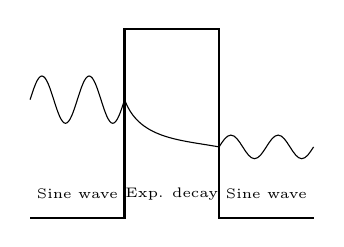
\begin{tikzpicture}[scale=0.6]
    % Border
    \draw[thick] (0,0) -- (2,0) -- (2,4) -- (4,4) -- (4,0) -- (6,0);
    
    % Sine waves
    \draw (0,2.5) sin (0.25,3.0) cos (0.5,2.5) sin (0.75,2.0) cos (1,2.5) sin (1.25,3.0) cos (1.5,2.5) sin (1.75,2.0) cos (2,2.5);
    \draw (2,2.5) to[out=290,in=170] (4,1.5);
    \draw (4,1.5) sin (4.25,1.75) cos (4.5,1.5) sin (4.75,1.25) cos (5,1.5) sin (5.25,1.75) cos (5.5,1.5) sin (5.75,1.25) cos (6,1.5);
    
    % Text
    \node at (1,0.5) {\tiny Sine wave};
    \node at (3,0.5) {\tiny Exp. decay};
    \node at (5,0.5) {\tiny Sine wave};
    
\end{tikzpicture}